\documentclass[11pt,handout,aspectratio=169,dvipsnames]{beamer}

\usepackage{listings}
\lstset{
    language=R,                     % Specify R as the programming language
    basicstyle=\ttfamily\scriptsize,      % Set font to typewriter (\ttfamily) and small size
    keywordstyle=\color{blue},       % Color for R keywords
    commentstyle=\color{gray},       % Color for comments
    stringstyle=\color{red},         % Color for strings
    numbers=left,                    % Line numbers on the left
    numberstyle=\tiny\color{gray},   % Small gray line numbers
    stepnumber=1,                     % Number every line
    breaklines=true,                 % Line breaking enabled
%    frame=single,                    % Single-line frame around code
    captionpos=b,                     % Caption position at bottom
    tabsize=2                         % Set tab size to 2 spaces
}
\usepackage{multirow}
\usepackage{tikz}
\usetikzlibrary{arrows,shapes}

%%%%%%%%% GENERAL PACKAGES
%\usepackage{xcolor}
%\usepackage{pdfpages}
%\usetheme[progressbar=frametitle]{metropolis}
%\setbeamercolor{background canvas}{bg=white}
%\usepackage{appendixnumberbeamer}
%\usepackage{booktabs}
%\usepackage[scale=2]{ccicons}
%\usepackage{pgfplots}
%\usepgfplotslibrary{dateplot}
%\usepackage{xspace}
%\newcommand{\themename}{\textbf{\textsc{metropolis}}\xspace}
%\usepackage[absolute,overlay]{textpos}

%%%%%%%%% COLOR THEME

% Define some colors:
\definecolor{DarkFern}{HTML}{407428}
\definecolor{DarkCharcoal}{HTML}{4D4944}
\definecolor{AlertColor}{RGB}{89,124,158}
\definecolor{HighLight}{RGB}{96,95,134}
\definecolor{Important}{RGB}{234,122,133}
\definecolor{Yellow}{HTML}{00539C}
\colorlet{Fern}{DarkFern!85!white}
\colorlet{Charcoal}{DarkCharcoal!85!white}
\colorlet{LightCharcoal}{Charcoal!50!white}
\colorlet{HighLight2}{AlertColor}
\colorlet{DarkRed}{red!70!black}
\colorlet{DarkBlue}{blue!70!black}
\colorlet{DarkGreen}{green!70!black}
\definecolor{RoyalBlue}{HTML}{00539C}
\definecolor{Peach}{HTML}{EEA47F}
\definecolor{ForestGreen}{HTML}{2C5F2D}
\definecolor{MossGreen}{HTML}{E8FCC9}
% Use the colors:
\setbeamercolor{title}{fg=Fern}
\setbeamercolor{frametitle}{fg=MossGreen,bg=ForestGreen}
\setbeamercolor{normal text}{fg=Charcoal!70!black}
\setbeamercolor{block title}{fg=black,bg=Fern!25!white}
\setbeamercolor{block body}{fg=black,bg=Fern!10!white}
\setbeamercolor{block title alerted}{fg=black,bg=DarkRed!25!white}
\setbeamercolor{block body alerted}{fg=black,bg=DarkRed!10!white}
\setbeamercolor{alerted text}{fg=DarkRed}
\setbeamercolor{itemize item}{fg=Charcoal}



%%%%%%%%% OTHER COMMANDS
\newcommand{\indep}{\perp\!\!\! \perp}
\newcommand{\comment}[1]{}
\newcommand{\bs}{\boldsymbol}
\newcommand{\tr}{\text{trace}}
\newcommand{\sgn}{{\rm sgn}}
\def\T{\top}
%\newcommand{\det}{\text{det}}
\newcommand{\var}{\mathrm{var}}
\newcommand{\cC}{{\cal C}}
\newcommand{\cG}{{\cal G}}
\newcommand{\cV}{{\cal V}}
\newcommand{\cE}{{\cal E}}
\newcommand{\cM}{{\cal M}}
\newcommand{\cP}{{\cal P}}
\newcommand{\cX}{{\cal X}}
\newcommand{\cY}{{\cal Y}}
\newcommand{\X}{\mathbf{X}}
\newcommand{\Y}{\mathbf{Y}}
\newcommand{\x}{\mathbf{x}}
\newcommand{\y}{\mathbf{y}}
\newcommand{\z}{\mathbf{z}}

\newcommand{\argmin}{\operatornamewithlimits{argmin}}
\newcommand{\eps}{\varepsilon}
\newcommand{\<}{\langle}
\renewcommand{\>}{\rangle}


\setbeamertemplate{itemize subitem}{\tiny\raise1.5pt\hbox{\donotcoloroutermaths$\blacktriangleright$}}
\setbeamertemplate{itemize subsubitem}{\tiny\raise1.5pt\hbox{\donotcoloroutermaths$\blacktriangleright$}}
\setbeamertemplate{enumerate item}{\insertenumlabel.}
\setbeamertemplate{enumerate subitem}{\insertenumlabel.\insertsubenumlabel}
\setbeamertemplate{enumerate subsubitem}{\insertenumlabel.\insertsubenumlabel.\insertsubsubenumlabel}
\setbeamertemplate{enumerate mini template}{\insertenumlabel}

\newcommand{\TODO}[1]{{\color{red}{[TODO: #1]}}}


\newcommand{\R}{\mathbb R}
\newcommand{\E}{\mathbb E}
\renewcommand{\P}{\mathbb P}


\DeclareMathOperator*{\cov}{cov}


\newsavebox{\zerobox}
\newenvironment{nospace}
{\par\edef\theprevdepth{\the\prevdepth}\nointerlineskip
  \setbox\zerobox=\vtop to 0pt\bgroup
  \hrule height0pt\kern\dimexpr\baselineskip-\topskip\relax
}
{\par\vss\egroup\ht\zerobox=0pt \wd\zerobox=0pt \dp\zerobox=0pt
  \box\zerobox}

\usepackage{soul}
\makeatletter
\let\HL\hl
\renewcommand\hl{%
  \let\set@color\beamerorig@set@color
  \let\reset@color\beamerorig@reset@color
  \HL}
  \makeatother


\title[STA437-Week1]{STA 437/2005: \\ Methods for Multivariate Data}
\subtitle[]{Week 11-12: Conditional independence and graphical models}
\author[Piotr Zwiernik]{Piotr Zwiernik}
\institute[UofT]{University of Toronto}
\date{}


%\usepackage{Sweave}

\begin{document}

\maketitle

\begin{frame}[plain,noframenumbering]{}
\begin{center}
	{\Huge \textcolor{DarkRed}{Conditional independence}}
\end{center}
\end{frame}

\begin{frame}[plain,noframenumbering]{}
\begin{center}
	{\huge \textcolor{DarkRed}{Basic definitions}}
\end{center}
\end{frame}

\begin{frame}{Random vector and independence}
	Let $(X,Y)$ be a vector of two random variables.
	\begin{alertblock}{Joint distribution}
		\textcolor{SeaGreen}{Density function} $f_{XY}(x,y)$ if continuous.\\[.1cm]
		\textcolor{SeaGreen}{Probability mass function} $f_{XY}(x,y)=\P(X=x,Y=y)$ if discrete.
	\end{alertblock}
		\begin{alertblock}{Marginal distribution}
continuous:\;\;\;$f_X(x)=\int_\R f_{XY}(x,y){\rm d}y$.\\[.1cm]
discrete:\;\;\;$f_X(x)=\sum_y f_{XY}(x,y)=\P(X=x)$.
	\end{alertblock}
	This can be generalized to random vectors.
\end{frame}

\begin{frame}{Independence}
\begin{beamercolorbox}[wd=\paperwidth,sep=2pt]{goldbox}
	If $f_{XY}(x,y)$ is the joint density (or PMF) of $(X,Y)$ then $X$ and $Y$ are independent if and only if \\[-.5cm] $$ f_{XY}(x,y)=f_X(x)f_Y(y)\qquad\mbox{for all }x,y.$$
		We write \alert{$X\indep Y$}.	
\end{beamercolorbox}
		Recall:
		$$
		\cov(X,Y)=\E(XY)-\E(X)\E(Y)\quad\mbox{and}\quad \var(X)=\cov(X,X).
		$$
		The correlation $\rho_{X,Y}$ between $X,Y$ is:
		$$
		\rho_{X,Y}\;=\;\tfrac{\cov(X,Y)}{\sqrt{\var(X)\var(Y)}}\;\in\;[-1,1].
		$$
		\begin{beamercolorbox}[wd=\paperwidth,sep=2pt]{important}
			If $X\indep Y$ then $\rho_{X,Y}=0$.\\ {\footnotesize(but in general not the other way around, see slide \ref{zerocor})}
		\end{beamercolorbox}
\end{frame}

\begin{frame}{Conditional distribution}
	\begin{block}{Conditional distribution}
		In the discrete case the conditional probability mass function is defined as
		$$f_{X|Y}(x|y)=\textcolor{DarkRed}{\P(X=x|Y=y)}=\tfrac{\P(X=x,Y=y)}{\P(Y=y)}  $$ 
		for all  $x,y$ such that  $\P(Y=y)>0$ and so $$f_{X|Y}(x|y)=\tfrac{f_{XY}(x,y)}{f_Y(y)} \mbox{ for all } x,y \mbox{ s.t. }f_Y(y)>0. $$ \textbf{In the continuous	case we use the same definition.}\end{block}
		\begin{alertblock}{Important reformulation of independence}
			$X\indep Y$ if and only if $f_{X|Y}(x|y)=f_X(x)$.\\
			(knowing $Y$ brings no extra information about $X$)
		\end{alertblock}

\end{frame}


\begin{frame}{A cautionary note}

	\begin{beamercolorbox}[wd=\paperwidth,sep=2pt]{notabene}	
Note: Large $f_{X|Y}(x|y)$ does not imply large $f_{Y|X}(y|x)$.\\[.5cm] 
\textbf{Example:} A medical test for a disease $D$ has outcomes + and - with probabilities\\ 
{\centering\begin{tabular}{l|ll}
  & $D$  & $D^c$ \\ \hline
+ & .009 & .099  \\
- & .001 & .891 
\end{tabular}\\}
\bigskip

As needed $\P(+|D)=0.9$ and $\P(-|D^c)= 0.9$. However, $\P(D|+)\approx 0.08$ (!)
 \end{beamercolorbox}
\end{frame}

%
%
%\begin{frame}{Appendix: Conditional expectation}
%Let $X,Y$ have joint distribution $f_{XY}(x,y)$ and conditional $f_{X|Y}(x|y)$. Then the \textcolor{SeaGreen}{conditional expectation} $\E[X|Y]$ is the expectation of $X$ with respect to the conditional distribution $X|Y=y$.
%$$
%\E[X|Y=y]\;\;=\;\;\begin{cases}
%	\sum_x x \,f_{X|Y}(x|y)\\
%	\int_\R x \,f_{X|Y}(x|y){\rm d}x
%\end{cases}.
%$$ 
%It is clear that $\E[g(Y)X|Y]=g(Y)\E[X|Y]$.\\[.2cm]
%\textbf{Note that $\E[X|Y]$ is a function of $Y$ and so a random variable!}\\[.2cm]
%A powerful result states that $$\E\big[\E(X|Y)\big]\;=\;\E(X).$$ 	
%\vspace{-.4cm}\begin{alertblock}{Example: two binary variables}
%	Suppose $f_{XY}(0,0)=0.4$, $f_{XY}(0,1)=0.2$, $f_{XY}(1,0)=0.1$, $f_{XY}(1,1)=0.3$. Then\ldots
%\end{alertblock}
%\end{frame}
%


\begin{frame}{Conditional independence}
	$X,Y,Z$ random variables.\\[.3cm]
	\alert{$X$ is independent of $Y$ given $Z$} (write \textcolor{SeaGreen}{$X\indep Y|Z$}) if
	$$
	f_{XY|Z}(x,y|z)\;=\;f_{X|Z}(x|z)f_{Y|Z}(y|z)\qquad\mbox{for every }z.
	$$
%	We can define conditional expectation $\E(X|Z)$ and \alert{conditional correlation} :$$
%	\rho_{X,Y| Z}\;:=\;\tfrac{\cov(X,Y|Z)}{\sqrt{\var(X|Z)\var(Y|Z)}}
%	$$
%	\textbf{Note that these are functions of $Z$!}\\[.3cm]
%	
%	If $X\indep Y|Z$ \quad then\quad  $\rho_{X,Y| Z}\equiv 0$\\
%	\footnotesize{(but not the other way around)}
		\begin{alertblock}{Important reformulation of independence}
			$X\indep Y|Z$ if and only if $f_{X|Y,Z}(x|y,z)=f_{X|Z}(x|z)$.\\
			(if we observed $Z$, extra information about $Y$ brings no extra information about $X$)
		\end{alertblock}
\end{frame}

%\begin{frame}{Partial correlation}
%In practice we often work with the partial correlation:
%	$$
%	\rho_{X,Y\cdot Z}\;:=\;\tfrac{\rho_{X,Y}-\rho_{X,Z}\rho_{X,Y}}{\sqrt{(1-\rho_{X,Z}^2)(1-\rho_{Y,Z}^2)}}.
%	$$
%	We have $\rho_{X,Y\cdot Z}=0$ if and only if in the \textbf{linear} regression of $X$ on $Y,Z$ the coefficient of $Y$ is zero.
%	\begin{beamercolorbox}[wd=\paperwidth,sep=5pt]{important}	
%		We have $\rho_{X,Y\cdot Z}=\rho_{X,Y|Z}$ in the case of \textcolor{SeaGreen}{Gaussian}, elliptical, multinomial and Dirichlet distributions. But not in general.
%	\end{beamercolorbox}
%
%	\textbf{Important}: If  $\bs X=(X_1,\ldots,X_m)$ is a random vector with covariance matrix $\Sigma$, denote $K=\Sigma^{-1}$, then for each $i,j\in \{1,\ldots,m\}$ 
%	$$
%	\rho_{X_i,X_j\cdot X_{\{1,\ldots,m\}\setminus \{i,j\}}}\;=\;-\tfrac{K_{ij}}{\sqrt{K_{ii}K_{jj}}}.
%	$$ 
%	So normalizing the \textbf{concentration matrix} gives the partial correlations.
%	\begin{itemize}
%		\item $\rho_{X_i,X_j\cdot X_{\{1,\ldots,m\}\setminus \{i,j\}}}=0$ \quad$\Longleftrightarrow$\quad $K_{ij}=0$
%		\item $\rho_{X_i,X_j\cdot X_{\{1,\ldots,m\}\setminus \{i,j\}}}\geq 0$ \quad$\Longleftrightarrow$\quad $K_{ij}\leq 0$
%	\end{itemize} 
%\end{frame}


\subsection{Testing independence}
\begin{frame}[plain,noframenumbering]{}
\begin{center}
	{\huge \textcolor{DarkRed}{Testing independence}}
\end{center}
\end{frame}

\begin{frame}{Recall: A statistical test}
	Given a statistical hypothesis $H_0:$ $\theta\in \Theta_0$, $H_1:$ $\theta\in \Theta_1$, a statistical test consists of a \textcolor{SeaGreen}{test statistics} $T(X^{(1)},\ldots,X^{(n)})$ and a \textcolor{SeaGreen}{rejection region}, typically of the form
	$$
	R\;=\;\{T(X^{(1)},\ldots,X^{(n)})>t\}.
	$$ 
\begin{beamercolorbox}[wd=\paperwidth,sep=2pt]{notabene}	
If the null hypothesis is true $T$ is unlikely to take large values. \end{beamercolorbox}
\begin{alertblock}{Type I error:\quad $\P(T\in R|H_0)$} 
	although $H_0$ is true, it is rejected 
\end{alertblock}
\begin{alertblock}{Type II error:\quad $\P(T\notin R|H_1)$} 
	although $H_0$ is false, it is retained\end{alertblock}
\noindent A good test should minimize probabilities of both types of errors.\\[.2cm]
%\begin{beamercolorbox}[wd=\paperwidth,sep=2pt]{important}	
%The idea is that $T$ has some known distribution under $H_0$ so that we can compute the probability of $T\in R$ easily. \end{beamercolorbox}
\end{frame}

%\begin{frame}{Some vocabulary}
%\textcolor{SeaGreen}{Power function}: \quad $\beta(\theta)=\P_\theta(T(X_1,\ldots,X_n)\in R )$\\[.4cm]
%\textcolor{SeaGreen}{Size of a test}: \quad $\sup_{\theta\in \Theta_0}\beta(\theta)$ (want this small to minimize type I error)\\[.4cm]
%A test has \textcolor{SeaGreen}{level $\alpha$} if size is $\leq \alpha$.\\[.4cm]
%%\textcolor{SeaGreen}{Uniformly most powerful test}: (uniformly) highest power under $H_1$ among all size $\alpha$ tests, that is $\beta(\theta)\geq\beta'(\theta)$ for all $\theta\in \Theta_1$ and all tests $\beta'$.\\[.4cm]
%%\textcolor{SeaGreen}{Simple hypothesis}: \quad $H_0$: $\theta=\theta_0$, $H_1$: $\theta\neq \theta_0$.\\[.4cm]
%\end{frame}

%\begin{frame}[label={exgauss}]{Example: Zero mean in the Gaussian distribution}
%Let $X_1,\ldots,X_n$ be a sample from $N(\mu,1)$. We test $H_0$: $\mu=0$ versus $H_1$: $\mu\neq 0$ (simple hypothesis)\\[.4cm]
%Intuitively, if $|\bar X_n|$ is ``large'', we should reject $H_0$. Note that under $H_0$ we have $\sqrt{n}\bar X_n\sim N(0,1)$.\\[.4cm]
%The idea is to propose a test statistic with a known distribution (under $H_0$) so that computations are easy. In our case let: $$T(X_1,\ldots,X_n)\;=\; \left|\sqrt{n}\bar X_n\right|.$$
%We get a $\alpha$ level test when $t=z_{\alpha/2}$.\\[.2cm] For example, for $\alpha=0.05$ and $\alpha'=0.01$ we get \texttt{qnorm(1-0.05/2)}=1.96 and \texttt{qnorm(1-0.01/2)}=2.58. 
%\end{frame}

%\begin{frame}{$p$-value}
%	If $\alpha'<\alpha$ then a level $\alpha'$ test has ``smaller'' rejection regions than a level $\alpha$ test. If we reject at level $\alpha$ then we also reject at level $\alpha'$.\\[.2cm]
%	$\bullet$ The level $\alpha'$ test is more \textcolor{SeaGreen}{conservative}.\\[.4cm]
%	For a given data there exists a smallest $\alpha$ that leads to rejection. This $\alpha$ is called the \textcolor{SeaGreen}{p-value}.\\[.2cm]
%	$\bullet$ In the example on slide~\ref{exgauss}, suppose we observed $T=2.1$. Then the p-value is:\;\; 2(1-\texttt{pnorm}(2.1))=0.036.\\[.2cm]
%	$\bullet$ p-value is the same as the probability of the test statistic being greater than its observed value. We want this probability to be small. By convention smaller than $0.05$ is significant.\\[.4cm] 
%	\begin{beamercolorbox}[wd=\paperwidth,sep=3pt]{important}	
%Note: The p-value is not the probability that the null hypothesis is true, or the probability that the alternative hypothesis is false.
% \end{beamercolorbox}
%\end{frame}


\begin{frame}{Testing independence}
Data: $(X_1,Y_1)$, \ldots, $(X_n,Y_n)\overset{iid}{\sim}P_{X,Y}$.\\[.3cm]
Goal: Decide whether $X\indep Y$.\\[.3cm]
Statistical test: \qquad $H_0:X\indep Y$,\quad $H_A:X\indep\!\!\!\!\!\!\not\;\;\; Y$\\[.7cm]
%\quad test statistics $T_n$ maps sample to $\R$\\[.1cm]
%\quad if $T> c$ we reject the null hypothesis\\[.1cm]
%\quad $c$ chosen to control the type I error	
There are many tests of independence.\\[.3cm]
We discuss some examples.
\end{frame}

\begin{frame}[fragile]{Test for vanishing correlation}
\begin{alertblock}{Fisher's z-transform test for Gaussian data}
Let $r_n$ is the sample correlation coefficient from an \emph{iid} sample $(X^{(i)},Y^{(i)})$.\\[.2cm] Define $Z_n=\tfrac{1}{2}\log\left(\tfrac{1+r_n}{1-r_n}\right)$.\\[.2cm] 
If $(X,Y)$ is bivariate normal with correlation $\rho$ then $Z_n$ has \alert{asymptotically} normal distribution with mean $\tfrac{1}{2}\log\left(\tfrac{1+\rho}{1-\rho}\right)$ and variance $\tfrac{1}{n-3}$.\\[.2cm]
%   \begin{lstlisting}
%# illustrate the normal approximation
%library(MCMCpack); n <- 1000; iter <- 1000; rho <- 0.2
%srho <- rep(0,iter)
%for (i in 1:iter) {srho[i] <- cor(mvrnorm(n,c(0,0),matrix(c(1,rho,rho,1),2,2)))[1,2]}
%hist(log((1+srho)/(1-srho))/2,prob=TRUE,ylim=c(0,13))
%curve(dnorm(x, mean=log((1+rho)/(1-rho))/2, sd=1/sqrt(n-3)), add=TRUE)
% \end{lstlisting}
 \end{alertblock}
 Fisher's z-transform test is implemented in \textsc{R} as \texttt{cor.test}.\\[4mm]
Non-gaussianity may invalidate the test and affect its power.	
\end{frame}

%\begin{frame}{}
%Compare the sample distribution of $Z_n$ with its theoretical asymptotic distribution.
%\begin{center}
%	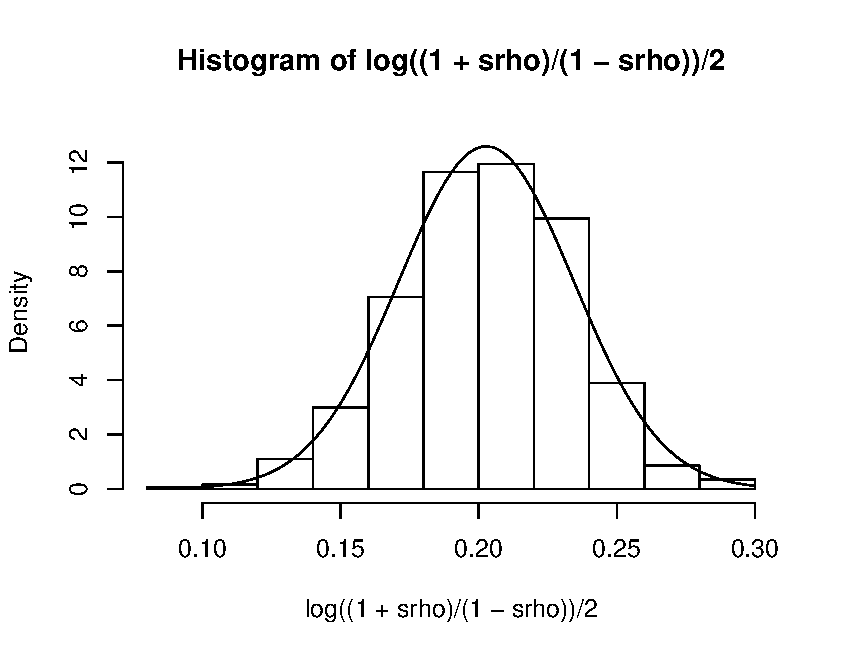
\includegraphics[scale=0.7]{pics/fisher_rho_hist}
%\end{center}	
%\end{frame}

%\begin{frame}[fragile]{}
%Fisher's z-transform test is implemented in \textsc{R} as \texttt{cor.test}.
%   \begin{lstlisting}
%> set.seed(1); n <- 100; rho <- 0.2
%> x <- mvrnorm(n,c(0,0),matrix(c(1,rho,rho,1),2,2))
%> cor.test(x[,1], x[,2], method = "pearson") 
%# Pearson's product-moment correlation
%data:  x[, 1] and x[, 2]
%t = 6.2913, df = 998, p-value = 4.704e-10
%alternative hypothesis: true correlation is not equal to 0
%95 percent confidence interval:
% 0.1349527 0.2542267
%sample estimates:
%      cor 
%0.1953118 
% \end{lstlisting}
%Try the same with $\rho=0$.\\[.2cm]
%\begin{beamercolorbox}[wd=\paperwidth,sep=5pt]{important}
%Non-gaussianity may invalidate the test and affect its power.	
%\end{beamercolorbox}
%\end{frame}

\begin{frame}[fragile,label=tau]{Basic nonparametric test}
\begin{block}{Kendall's tau test for non-Gaussian data}
Suppose a bivariate sample $(x_i,y_i)$ for $i=1,\ldots,n$ is given.\\[.2cm]
Pair $(x_i,y_i)$ , $(x_j,y_j)$ is \alert{concordant} if $(x_i,y_i)< (x_j,y_j)$ or $(x_i,y_i)> (x_j,y_j)$. Otherwise  \alert{discordant}.\\[.2cm]
Define $\tau_{XY}\;=\;\tfrac{(\#\mbox{concordant})-(\#\mbox{discordant})}{{n\choose 2}}\;\in\;  [-1,1]$.\\[.2cm]
Test based on Kendell's $\tau$ statistic is implemented in \textsc{R} as \texttt{cor.test}.
   \begin{lstlisting}
> set.seed(1); n <- 200; rho <- 0.2; Z <- runif(n); 
> X <- runif(n)^2+sqrt(rho)*Z; Y <- runif(n)+sqrt(rho)*Z
> cor.test(X, Y, method = "pearson")$p.value
[1] 0.03417231
> cor.test(X, Y, method = "kendall")$p.value
[1] 0.01100592
 \end{lstlisting}
\end{block}
$\tau_{XY}$ is asymptotically normal under independence, which is used to construct p-values.
\end{frame}


\begin{frame}[fragile]{Non-Gaussianity issue}
\begin{beamercolorbox}[wd=\paperwidth,sep=5pt]{important}
Vanishing covariance does not imply independence!
\end{beamercolorbox}
\begin{lstlisting}
# generate sample from two uncorrelated but dependent random variables
> set.seed(1); n <- 200
> A <- runif(n)-1/2; B <- runif(n)-1/2
> X <- t(c(cos(pi/4),-sin(pi/4)) %*% rbind(A,B))
> Y <- t(c(sin(pi/4),cos(pi/4)) %*% rbind(A,B))
> cor.test(X,Y, method = "pearson")
# Pearson's product-moment correlation
data:  X and Y
t = -0.84711, df = 198, p-value = 0.398
alternative hypothesis: true correlation is not equal to 0
95 percent confidence interval:
 -0.1971897  0.0793095
sample estimates:
        cor 
-0.06009275 \end{lstlisting}
$X$ and $Y$ are uncorrelated but dependent!
\end{frame}

\begin{frame}{}
\begin{center}
	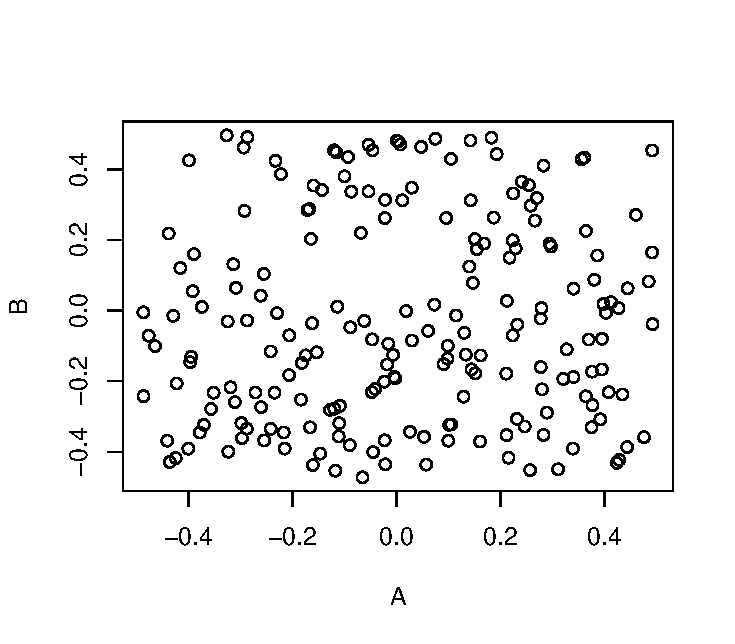
\includegraphics[width=0.5\textwidth]{pics/ABplot}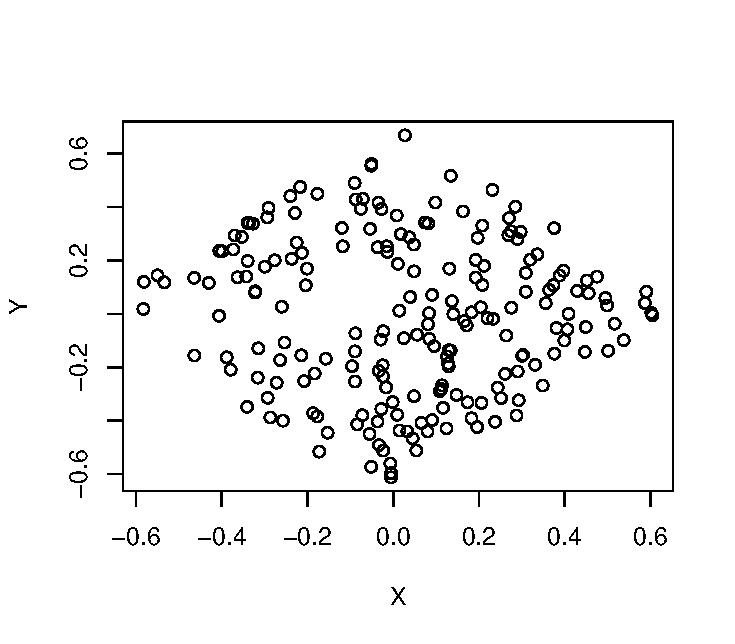
\includegraphics[width=0.5\textwidth]{pics/XYplot}	
\end{center}
	We see that $X$ and $Y$ are highly dependent. 
\end{frame}

\begin{frame}[fragile,label=zerocor]{Test based on distance correlation (very high level)}
\alert{Distance correlation} $\mathcal R(X,Y)$ provides a test which applies when 
$X$, $Y$ are two random \textbf{vectors} of any dimensions.\\[.2cm]
$\mathcal R(X,Y)=0$ if and only if $X$ and $Y$ are independent.\\[.2cm]
The sample version of $\mathcal R(X,Y)$ gives a \alert{nonparametric} test of independence. \\[.2cm]
%This is also implemented in R in package \texttt{energy}.
\begin{lstlisting}
> library(energy); set.seed(1); n <- 200
> A <- runif(n)-1/2; B <- runif(n)-1/2
> X <- t(c(cos(pi/4),-sin(pi/4)) %*% rbind(A,B))
> Y <- t(c(sin(pi/4),cos(pi/4)) %*% rbind(A,B))
> dcor.test(X,Y,R=1000)

# dCor independence test (permutation test)
data:  index 1, replicates 1000
dCor = 0.21161, p-value = 0.004995
sample estimates:
      dCov       dCor    dVar(X)    dVar(Y) 
0.03999654 0.21160982 0.17870935 0.19990601 
\end{lstlisting}
Tends to be more powerful than the test based on Kendall's tau.
\end{frame}

\begin{frame}[fragile]{Another cautionary example}
	Bowman\&Azzalini (1997) analyse aircraft wing span and speed data.	 \\[4mm]
%	\begin{center}
%	 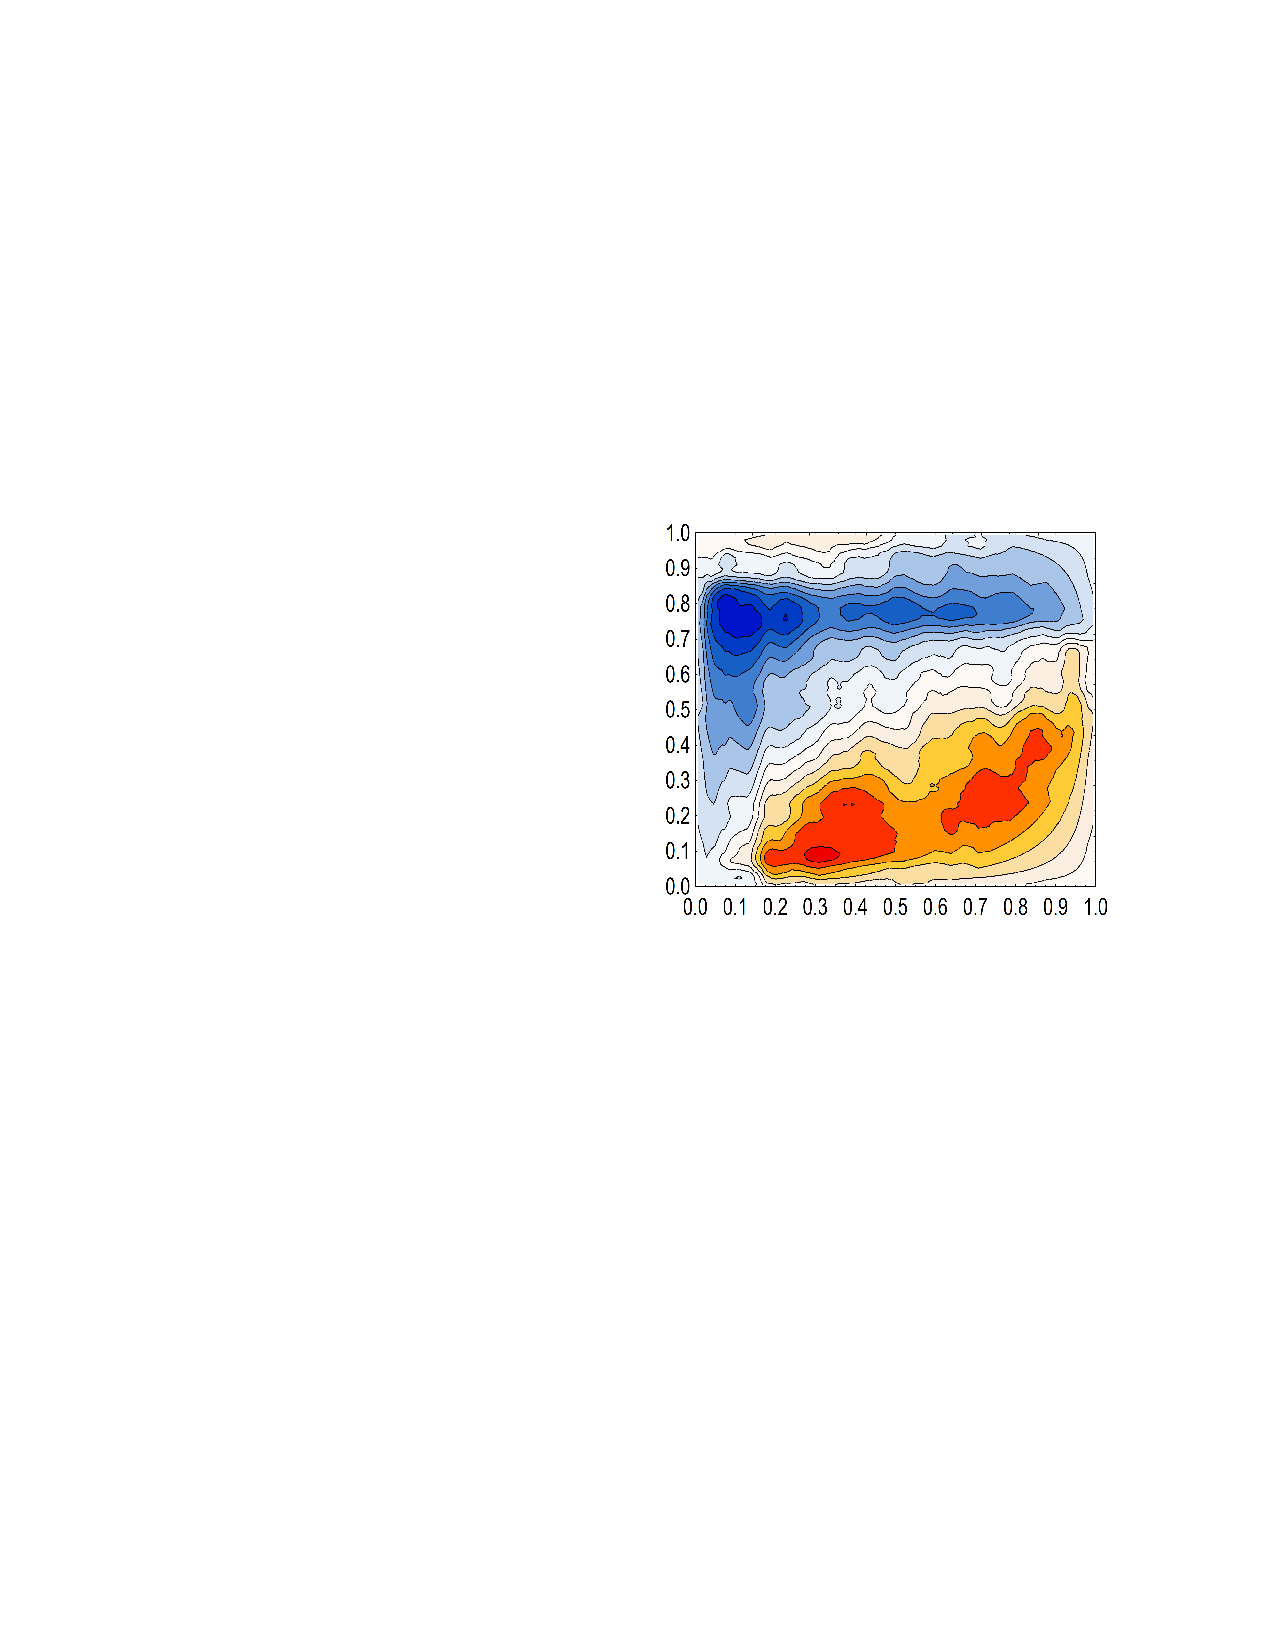
\includegraphics[scale=.5]{pics/aircraft}	 	
%	 \end{center}
	 \begin{lstlisting}
> library(sm); set.seed(1); 
> X <- aircraft$Span
> Y <- aircraft$Speed
> cor.test(X,Y)$p.value
[1] 0.7816014
> dcor.test(X,Y,R=1000)$p.value
[1] 0.000999001
\end{lstlisting}
\end{frame}

\begin{frame}{Appendix: Asymptotic Likelihood Ratio Test}
Consider a parametric model $\{\P_\theta: \theta\in \Theta\}$ and let $\Theta_0\subseteq \Theta$. Test \alert{$H_0:\theta^*\in\Theta_0$}.\\[4mm]
Let $\ell(\theta)=\sum_{i=1}^n\log f(\x_i;\theta)$ be the log-likelihood. Compute the statistics: 
$$
\lambda_n\;:=\;2(\sup_{\theta\in \Theta}\ell(\theta)-\sup_{\theta\in \Theta_0}\ell(\theta))
$$  
\begin{alertblock}{Wilks' theorem (simplified version)}
	Under $H_0$, if $\Theta$ and $\Theta_0$ are regular $\lambda_n\xrightarrow{d}\chi^2_d$, where d = $\dim(\Theta) - \dim(\Theta_0)$ is the difference in the number of parameters.
\end{alertblock}

\end{frame}

\begin{frame}{Testing independence for discrete distributions}
	\begin{block}{G-test}
In the context of count data the LRT is called the \alert{G-test}.\end{block}
\bigskip

\textbf{Example (Testing Independence)}:\\[4mm]
Suppose we have $X$ with $k$ possible values and $Y$ with $l$ possible values. \\[4mm]
	The saturated model for $(X,Y)$ has dimension $kl-1$.\\[4mm]
	The independence model $X\indep Y$ has dimension $(k-1)+(l-1)$.\\[4mm]
	We could use LRT with $d=(k-1)(l-1)$.


\end{frame}


\begin{frame}[fragile]{Tests for discrete data}
	\begin{alertblock}{$\chi^2$-test for discrete data (uses \texttt{library(DescTools)})}
   \begin{lstlisting}
> M <- as.table(rbind(c(762, 327, 468), c(484, 239, 477)))
> dimnames(M) <- list(gender = c("F", "M"),
+                     party = c("Democrat","Independent", "Republican"))

# Perform the LRT (G-test)
> GTest_result <- GTest(M)
# Print results
> print(GTest_result)

Log-likelihood ratio (G-test) test of independence without correction

data:  M
G = 30.017, X-squared df = 2, p-value = 3.034e-07
      \end{lstlisting}
\end{alertblock}
\texttt{df = 2} is the difference between $5$ (saturated model) and $3$ (independence)
\end{frame}

\begin{frame}[plain,noframenumbering]{}
\begin{center}
	{\huge \textcolor{DarkRed}{Testing conditional independence}}
\end{center}
\end{frame}


\begin{frame}[fragile]{Testing conditional independence}
Testing conditional independence is hard in general.\\[.2cm] 
(For discrete data we use the LRT.)\\[.2cm]

Some parametric tests are implemented in the library \texttt{bnlearn}.\\
Many non-parametric methods have been implemented in \texttt{CondIndTest}
 \begin{lstlisting}
> library(CondIndTests); library(bnlearn); set.seed(1); n <- 100
> Z <- rnorm(n); X <- 4 + 2 * Z + rnorm(n); Y <- 3 * X^2 + Z + rnorm(n)
> CondIndTest(X,Y,Z, method = "KCI")$pvalue 
[1] 2.419926e-10
> bnlearn::ci.test(X,Y,Z)$p.value 
[1] 1.15458e-25
\end{lstlisting}
\medskip

{\scriptsize See Section 3 in: 
C. Heinze-Deml, J. Peters, N. Meinshausen, Invariant Causal Prediction for Nonlinear Models, Journal of Causal Inference, 2018.}
\bigskip

{\scriptsize See: \url{http://www.bnlearn.com/documentation/man/conditional.independence.tests.html}}
\end{frame}

\begin{frame}[label=SP]{Simpson's paradox: UC Berkeley admissions example}
		The admission figures of the grad school at UC Berkeley in 1973: 8442 (44\%) men, 4321 (35\%) women admitted.\\[.3cm] The same data conditioned on the department are:\\[.3cm]
\hspace{.7cm}\begin{tabular}{|c|c|c|c|c|}
\hline
\multirow{2}{*}{Department} & \multicolumn{2}{c|}{Men}   & \multicolumn{2}{c|}{Women} \\ \cline{2-5} 
                            & Applicants & Admitted       & Applicants & Admitted       \\ \hline
A                           & 825        & 62\%          & 108        & \textbf{82\%} \\ \hline
B                           & 560        & 63\%          & 25         & \textbf{68\%} \\ \hline
C                           & 325        & \textbf{37\%} & 593        & 34\%          \\ \hline
D                           & 417        & 33\%          & 375        & \textbf{35\%} \\ \hline
E                           & 191        & \textbf{28\%} & 393        & 24\%          \\ \hline
F                           & 373        & 6\%           & 341        & \textbf{7\%}  \\ \hline
\end{tabular}
\medskip

``Measuring bias is harder than is usually assumed, and the evidence is sometimes contrary to expectation.''\\[.3cm] \tiny(Bickel et al,  \textit{Sex Bias in Graduate Admissions: Data From Berkeley}, Science, 1975) 
\end{frame}

\begin{frame}[fragile]{}
	In R:
	\begin{lstlisting}
> library(gRim); data(UCBAdmissions)
> gRim::ciTest(as.data.frame(UCBAdmissions),set=~Gender+Admit+Dept)

set: [1] "Gender" "Admit"  "Dept"  
Testing Gender _|_ Admit | Dept 
Statistic (DEV):    0.000 df: 6 p-value: 1.0000 method: CHISQ

Slice information:
  statistic p.value df Dept
1         0       1  1    A
2         0       1  1    B
3         0       1  1    C
4         0       1  1    D
5         0       1  1    E
6         0       1  1    F
 \end{lstlisting}
 In the last part a simple independence test is performed for each department separately. 
% \includegraphics[scale=.3]{pics/UCB1} \includegraphics[scale=.3]{pics/UCB2}
\end{frame}



%
%\begin{frame}[fragile,label=SP2]{Florida murderers}
%Sentences in 4863 murder cases in Florida over the six
%years 1973-78
%\begin{center}
%\begin{tabular}{lcc} \hline
%&\multicolumn{2}{c}{Sentence}\\
%\cline{2-3}
%Murderer&Death&Other\\
%\hline Black&59&2547\\ White&72&2185\\
%\hline
%\end{tabular}
%\end{center}
%The table shows a greater proportion
% of white murderers receiving death sentence than black
%(3.2\% vs.\ 2.3\%).
%	\begin{lstlisting}
%> flor <- matrix(c(59,72,2547,2185),2,2)
%> dimnames(flor) <- list(Murderer=c("Black","White"),Sentence=c("Death","Other"))
%> chisq.test(flor)
%
%Pearsons Chi-squared test with Yates continuity correction
%data:  flor
%X-squared = 3.6117, df = 1, p-value = 0.05737
%\end{lstlisting}
%\end{frame}
%
%\begin{frame}[fragile]{Controlling for colour of victim}
%\begin{center}
%\begin{tabular}{llcc}
%\hline
%&&\multicolumn{2}{c}{Sentence}\\
%\cline{3-4}
%Victim&Murderer&Death&Other\\
%\hline
%Black&Black&11&2309\\
%&White&0&111\\
%White&Black&48&238\\
%&White&72&2074\\
%\hline
%\end{tabular}
%\end{center}
%Now the table for given colour
%of victim shows a very different picture.
%
%
%%\pause
%\smallskip
%
% In particular,
%note that 111 white murderers killed black victims and
%none were sentenced to death.
%	\begin{lstlisting}
%> flor <- c(11,48,0,72,2309,238,111,2074); dim(flor) <- c(2,2,2)
%> dimnames(flor) <- list(Victim=c("Black","White"),Murderer=c("Black","White"),Sentence=c("Death","Other"))
%> ciTest_table(flor,set=~Sentence+Murderer+Victim)
%Testing Sentence _|_ Murderer | Victim 
%Statistic (DEV):   67.980 df: 2 p-value: 0.0000 method: CHISQ
% \end{lstlisting}
%\end{frame}
%

\subsection{Multivariate normal distribution}
\begin{frame}[plain,noframenumbering]{}
\begin{center}
	{\huge \textcolor{DarkRed}{Conditional independence for Gaussian distributions}}
\end{center}
\end{frame}



\begin{frame}{Recall: Marginal and conditional distributions}
	Split $X$ into two blocks $X=(X_A,X_B)$. Denote $$\mu=(\mu_A,\mu_B)\qquad\mbox{and}\qquad\Sigma=\begin{bmatrix}
		\Sigma_{AA} & \Sigma_{AB}\\
		\Sigma_{BA} & \Sigma_{BB}
	\end{bmatrix}.$$
	\begin{block}{Marginal distribution}
		$X_A\sim N_{|A|}(\mu_A,\Sigma_{AA})$
	\end{block}
	\begin{block}{Conditional distribution}
		$X_A|X_B=x_B\sim N_{|A|}\left(\textcolor{red}{\small \mu_A+\Sigma_{AB}\Sigma_{BB}^{-1}(x_B-\mu_B)},\textcolor{blue}{\small \Sigma_{AA}-\Sigma_{AB}\Sigma_{BB}^{-1}\Sigma_{BA}}\right)$
		\begin{itemize}
			\item Note that the conditional covariance is constant.
		\end{itemize}
	\end{block}
%	\bigskip
%	\textbf{Example}: Consider a bivariate normal with $\mu=(0,2)$ and $\Sigma=\begin{bmatrix}
%		1 & 0.7\\0.7 & 1
%	\end{bmatrix}$. We have  $\E[X_1|X_2]={0.7}(X_2-2)$\; and\; ${\rm var}(X_1|X_2)=1-{0.7^2}= 0.51 $.
\end{frame}


\begin{frame}{Conditional independence}
\begin{alertblock}{Independence and conditional independence}
$X_i\indep X_j$ if and only if $\Sigma_{ij}=0$.\\[.3cm]
$X_i\indep X_j|X_{C}$\;\; if and only if \;\; $\Sigma_{ij}-\Sigma_{i,C}\Sigma_{C,C}^{-1}\Sigma_{C,j}=0$\\[.3cm]
Let $R=V\setminus \{i,j\}$. The following are equivalent:
\begin{itemize}
	\item $X_i\indep X_j|X_{R}$
	\item $\Sigma_{ij}-\Sigma_{i,R}\Sigma_{R,R}^{-1}\Sigma_{R,j}=0$
	\item \textcolor{blue}{$(\Sigma^{-1})_{ij}=0$}
\end{itemize}
\end{alertblock}
{\tiny Useful: \url{https://en.wikipedia.org/wiki/Block_matrix\#Block_matrix_inversion}}
%\begin{beamercolorbox}[wd=\paperwidth,sep=2pt]{notabene}	
%Central Limit Theorem provides the biggest motivation for Gaussian distributions.\end{beamercolorbox}
\end{frame}


\section{Undirected graphical models}

\begin{frame}[plain,noframenumbering]{}
\begin{center}
	{\Huge \textcolor{DarkRed}{Undirected graphical models}}
\end{center}
\end{frame}


\subsection{Modelling with graphs}
\begin{frame}[plain,noframenumbering]{}
\begin{center}
	{\huge \textcolor{DarkRed}{Graph factorizations}}
\end{center}
\end{frame}

\begin{frame}{Factorization}
	$G=$ an undirected graph with nodes $\{1,\ldots,m\}$ and cliques $C_1,\ldots,C_k$.\\
	We say that density $f(\bs x)$ \textbf{\alert{factorizes according to $G$} }if for all $\bs x\in \cX$
	$$
	f(\bs x)\;=\;\phi_{C_1}(\bs x_{C_1})\cdots \phi_{C_k}(\bs x_{C_k}),
	$$ 
	where $\phi_C(\bs x_C)\geq 0$. 	(a notion of simplicity)\\[.3cm]
	
	\begin{alertblock}{For example}
		$$
	\tikzstyle{vertex}=[circle,fill=black,minimum size=5pt,inner sep=0pt]
\tikzstyle{hidden}=[circle,draw,minimum size=5pt,inner sep=0pt]
  \begin{tikzpicture}[scale=.6,baseline=5mm]
  \node[vertex] (1) at (0,2)  [label=left:$1$] {};
    \node[vertex] (2) at (2,2) [label=right:$2$]{};
    \node[vertex] (3) at (2,0) [label=right:$3$]{};
    \node[vertex] (4) at (0,0) [label=left:$4$]{};
     \draw[line width=.3mm] (2) to (1);
    \draw[line width=.3mm] (3) to (2);
    \draw[line width=.3mm] (3) to (4);
    \draw[line width=.3mm] (4) to (1);
    \draw[line width=.3mm] (1) to (3);
  \end{tikzpicture}\qquad f(\bs x)=\phi_{123}(x_1,x_2,x_3)\phi_{134}(x_1,x_3,x_4).
	$$
	\end{alertblock}
\hl{Exercise:} This gives an alternative characterisation of $X_2\indep X_4|(X_1,X_3)$.
\end{frame}

\begin{frame}[label=HC]{Hammersley-Clifford theorem}
Let $f>0$ be a dentity function for $\bs X=(X_1,\ldots,X_m)$. Then the following are equivalent:\\[.3cm]
\begin{enumerate}
	\item [(F)] $f$ factorizes according to $G$. \\[.4cm]
	\item [(G)] $X_A\indep X_B|X_C$ whenever $C$ \alert{separates} $A$ and $B$ in $G$.\\[.4cm]
	\item [(P)] $X_i\indep X_j|X_{V\setminus \{i,j\}}$ whenever $i,j$ not connected by an edge in $G$.
\end{enumerate}
\bigskip

The graph represents conditional independence.\\[.5cm]

\end{frame}


\begin{frame}{Graphical model $\cM(G)$}
	$G$ a graph with $m$ nodes representing a random vector $X=(X_1,\ldots,X_m)$.\\[.3cm]
	\begin{alertblock}{Definition (Graphical model $\cM(G)$)}
		$\cM(G)$ is the family of all distributions of $X$ that factorize according to $G$.
	\end{alertblock}
	By the Hammersley-Clifford theorem this can be equivalently described by conditional independences. (we work with positive distributions only)
	\bigskip
	
	Model families that admit suitable factorizations are described in later parts:
\begin{enumerate}
	\item \textcolor{SeaGreen!80!black}{log-linear models} for multivariate discrete data
	\item graphical \textcolor{SeaGreen!80!black}{Gaussian models} for multivariate Gaussian data.
\end{enumerate}
This drives modelling for more complicated (non-parametric) settings.
\end{frame}


\subsection{Gaussian graphical models}
\begin{frame}[plain,noframenumbering]{}
\begin{center}
	{\huge \textcolor{DarkRed}{Gaussian graphical models (GGMs)}}
\end{center}
\end{frame}


\begin{frame}{The Gaussian case}
\begin{block}{For a Gaussian distribution in $\cM(G)$:}
		The  non-edges of $G$ correspond to conditional independences $X_i\indep X_j|X_{V\setminus \{i,j\}}$ or equivalently \alert{$\mathbf{K_{ij}=0}$}.
%		\begin{itemize}
%			\item Indeed, $\rho_{ij|V\setminus \{i,j\}}=-\tfrac{K_{ij}}{\sqrt{K_{ii}K_{jj}}}$.
%		\end{itemize}
\end{block}
\hl{Exercise:} How $K_{ij}=0$ implies that the density factorizes into factors $V\setminus\{i\}$, $V\setminus \{j\}$.

\begin{alertblock}{Two main estimation problems:}
	Consider an \emph{iid} sample $\x_1,\ldots,\x_n$ from a distribution in $\cM(G)$.\\[.2cm]
\begin{enumerate}
	\item [(i)] Estimate $\Sigma$ for a fixed graph $G$.
	\item [(ii)] Learn the underlyin graph if it is unknown.
\end{enumerate} 
\end{alertblock}
\end{frame}


\begin{frame}[fragile,label=samplcov]{On concentration of the covariance matrix}
%	The covariance matrix has ${m+1\choose 2}$ parameters. 
	\begin{lstlisting}
> K <- matrix(c(1,0,1/2,0,1,1/2,1/2,1/2,1),3,3); Sig <- solve(K)
> set.seed(1)
> X10 <- mvrnorm(10,c(0,0,0),Sig); S10 <- cov(X10)
> X100 <- mvrnorm(100,c(0,0,0),Sig); S100 <- cov(X100)
> X1000 <- mvrnorm(1000,c(0,0,0),Sig); S1000 <- cov(X1000)
> solve(S10); solve(S100); solve(S1000)
          [,1]     [,2]      [,3]
[1,] 1.9379597 1.616762 0.8595338
[2,] 1.6167622 4.076235 2.1360457
[3,] 0.8595338 2.136046 1.6042403
           [,1]       [,2]      [,3]
[1,] 1.04792019 0.08406772 0.5781926
[2,] 0.08406772 0.93313405 0.3880432
[3,] 0.57819258 0.38804318 1.1148584
            [,1]        [,2]      [,3]
[1,]  0.88842341 -0.02029737 0.4710935
[2,] -0.02029737  0.90492134 0.4558757
[3,]  0.47109348  0.45587568 0.9628081\end{lstlisting}
Without regularization estimating a covariance matrix is a hard problem.\\[.2cm]
Estimating the graph seems easier! (at least in this favorable case)
\end{frame}

\begin{frame}{The Gaussian likelihood function}
	The sample covariance matrix of the sample $\x_1,\ldots,\x_n$ is
	$$S=\frac{1}{n}\sum_{i=1}^n(\x_i-\bar \x)(\x_i-\bar \x)^T.$$
Recall that the log-likelihood is
$$\log L(\mu,K)\;=\;\tfrac{n}{2}\log\det K-\tfrac{n}{2}\tr(KS)-\tfrac{n}{2}(\bar \x-\mu)^T K(\bar \x-\mu).$$
For fixed $K$ we get $\hat\mu=\bar \x$ giving the \alert{profile likelihood}
$$
\log L(\hat \mu,K)\;=\;\tfrac{n}{2}\log\det K-\tfrac{n}{2}\tr(KS).
$$
\end{frame}

\begin{frame}{Maximizing the likelihood over $\mathcal M(G)$}
$\cM(G)$ consists of PD matrices $K$ such that $K_{ij}=0$ for $ij\notin E$. \\[.3cm]

	Optimizing $\log L(\hat \mu,K)$ over $\cM(G)$ is a convex optimization problem.\\[.3cm]
	The MLE is the \textcolor{SeaGreen}{unique} point $\hat\Sigma$ (with $\widehat K=\widehat \Sigma^{-1}$) such that:
	\begin{enumerate}
		\item [(i)] $\hat\Sigma_{ii}=S_{ii}$ for all $i$, and $\hat\Sigma_{ij}=S_{ij}$ for all edges $ij\in G$,
		\item [(ii)] $\hat K_{ij}=0$ for all $ij\notin G$.
	\end{enumerate}
	\begin{alertblock}{Maximization}
		Typically numerically using a block \textcolor{SeaGreen}{coordinate-descent} scheme (\texttt{ggmfit}).
		%If $G$ is decomposable, the MLE admits a closed-form solution.
	\end{alertblock}
		\begin{block}{The deviance}
		Gives the likelihood ratio statistic to test against the unconstrained model. 
	\end{block}
\end{frame}

\begin{frame}[fragile]{Example: Financial market data}
	Using \texttt{gRbase}, \texttt{gRim}, \texttt{RBGL}:
\begin{lstlisting}
> data(EuStockMarkets)  # European stock market index data
> df <- as.data.frame(EuStockMarkets)  # Convert to a dataframe
> df <- scale(df)  # Standardize data
# Define graphical model structure (assumed dependencies)
> glist <- list(c("DAX", "SMI", "CAC"), c("SMI", "CAC", "FTSE"))
# Fit Gaussian graphical model
> gen.fit <- cmod(glist, data=df, fit=TRUE)
# Deviance and goodness-of-fit test
> gen.fit$fitinfo$dev; 1 - pchisq(gen.fit$fitinfo$dev, df=1)
[1] 0.6793619
[1] 0.4098065
# Visualize estimated partial correlation network
> K_sym <- (gen.fit$fitinfo$K + t(gen.fit$fitinfo$K)) / 2  
> qgraph::qgraph(-cov2cor(K_sym), directed = FALSE)   \end{lstlisting}
\end{frame}

\begin{frame}[plain,noframenumbering]{}
\begin{center}
	{\huge \textcolor{DarkRed}{Structure learning in GGMs}}
\end{center}
\end{frame}

\begin{frame}{Model selection methods}
How to learn the graph:\\[.4cm]
\begin{itemize}
	\item Stepwise methods,\\[.4cm]
	\item Convex optimization,\\[.4cm]
\end{itemize}	
\end{frame}


\begin{frame}{Appendix: Information criteria in model selection}
	Information criteria provide a popular method for model selection.\\[3mm] 
	Consider a selection of models $M_1,\ldots,M_r$ with dimensions $d_1,\ldots,d_r$.\\[3mm] 
	Given a sample $\x_1,\ldots,\x_n$, we compute the MLE for each of the models; $\ell(M_i)$ denotes the value of the log-likelihood.\\[3mm] 
	Then
	$$
	AIC_i\;=\;-2 \ell(M_i)+2 d_i
	$$
	$$
	BIC_i\;=\;-2 \ell(M_i)+\log(n) d_i
	$$
	We pick the model with the lowest Akaike Information Criterion (AIC) or Bayesian Information Criterion (BIC).
	\begin{alertblock}{Dimension of a Gaussian Graphical Model}
		For GGMs the dimension is simply $|V|+|E|$.
	\end{alertblock}
\end{frame}

\begin{frame}[fragile,label=carcass_stepwise]{Stepwise methods}
%	\begin{alertblock}{Stepwise backward model selection}
	The \texttt{stepwise} function in \texttt{gRim} performs stepwise model selection based on a variety of criteria (AIC, BIC, etc)	
	\begin{lstlisting}
sat.carc <- cmod(~.^.,data=carcass); n <- nrow(carcass)
test.carc <- stepwise(sat.carc,details=1,criterion="aic",type="decomposable",k=log(n))
# plot(test.carc) or using the qgraph package
Sigma.hat <- solve(test.carc$fitinfo$K)
qgraph::qgraph(Sigma.hat,graph="pcor") 
\end{lstlisting}
%	\end{alertblock}
%	\begin{alertblock}{BIC model selection}
%		s
%	\end{alertblock}
\begin{center}
%	{\tiny\begin{table}[ht]
%\centering
%\begin{tabular}{rrrrrrrr}
%  \hline
% & F11 & M11 & F12 & M12 & F13 & M13 & LM \\ 
%  \hline
%F11 & 0.44 & 0.02 & -0.20 & -0.07 & -0.16 & 0.05 & 0.10 \\ 
%  M11 & 0.02 & 0.16 & -0.03 & -0.06 & -0.04 & -0.05 & -0.03 \\ 
%  F12 & -0.20 & -0.03 & 0.54 & 0.06 & -0.20 & -0.04 & 0.09 \\ 
%  M12 & -0.07 & -0.06 & 0.06 & 0.14 & 0.00 & -0.09 & 0.00 \\ 
%  F13 & -0.16 & -0.04 & -0.20 & 0.00 & 0.55 & 0.00 & 0.07 \\ 
%  M13 & 0.05 & -0.05 & -0.04 & -0.09 & 0.00 & 0.16 & -0.02 \\ 
%  LM & 0.10 & -0.03 & 0.09 & 0.00 & 0.07 & -0.02 & 0.27 \\ 
%   \hline
%\end{tabular}
%\end{table}}
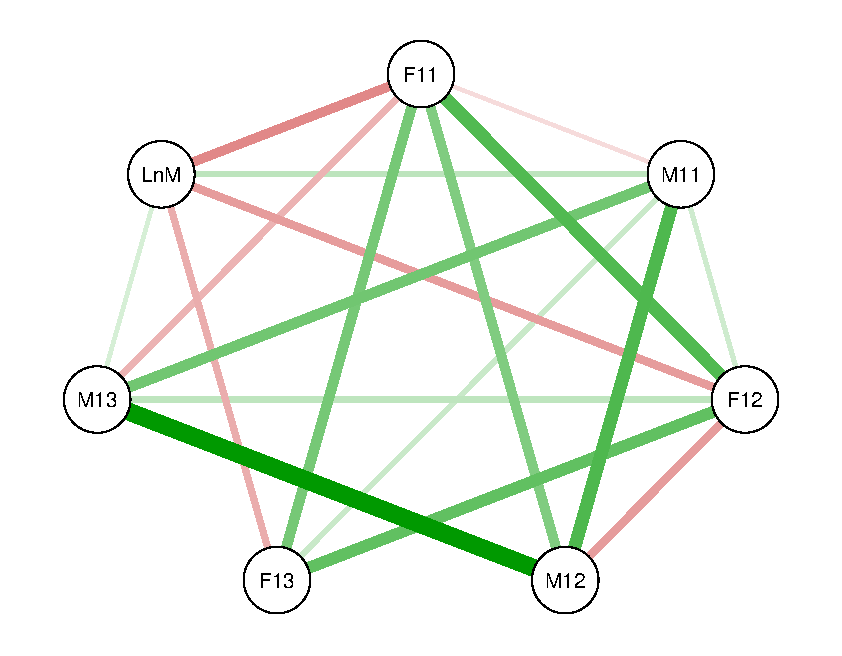
\includegraphics[scale=.4]{pics/carcass}
\end{center}
\end{frame}




\begin{frame}[fragile]{Learning the graph in high-dimension}
\begin{alertblock}{Graphical LASSO}
	If the dimension $m$ is large then the number of possible models is too large.\\[.2cm]


Instead, following the same idea as in the LASSO regression we maximize
$$
L_{\rm pen}(K,\hat \mu)\;=\;\log\det (K)-\tr(SK)-\alert{\lambda \|K\|_1},
$$
where $\|K\|_1=\sum_{i\neq j}|K_{ij}|$ and $\lambda$ is a fixed penalty parameter.
\end{alertblock}
\begin{block}{Implementation in R}
	See the packages \texttt{glasso} and \texttt{EBICglasso} (finds an optimal $\lambda$).
	\begin{lstlisting}
> S <- cor(data)
> lambda_opt <- 0.1  # Set a small regularization parameter
> glasso_fit <- glasso(S, rho=lambda_opt)
\end{lstlisting}
\end{block}

%\begin{block}{Example: Financial Networks (using \texttt{glasso,qgraph,quantmod})}
%\begin{lstlisting}
%symbols <- c("AAPL", "MSFT", "GOOG", "AMZN", "TSLA", "META", "NFLX", "NVDA", "JPM", "GS")
%getSymbols(symbols, from="2022-01-01", to="2023-01-01", src="yahoo")
%returns <- do.call(merge, lapply(symbols, function(sym) dailyReturn(Cl(get(sym)), type="log")))
%returns <- na.omit(returns)
%S <- cor(returns)
%
%\end{lstlisting}
%	The estimated graph has  137 edges compared to 496 of the full graph.
%\end{block}
\end{frame}

%\begin{frame}[plain,label=pers_lasso]{}
%	\begin{center}
%		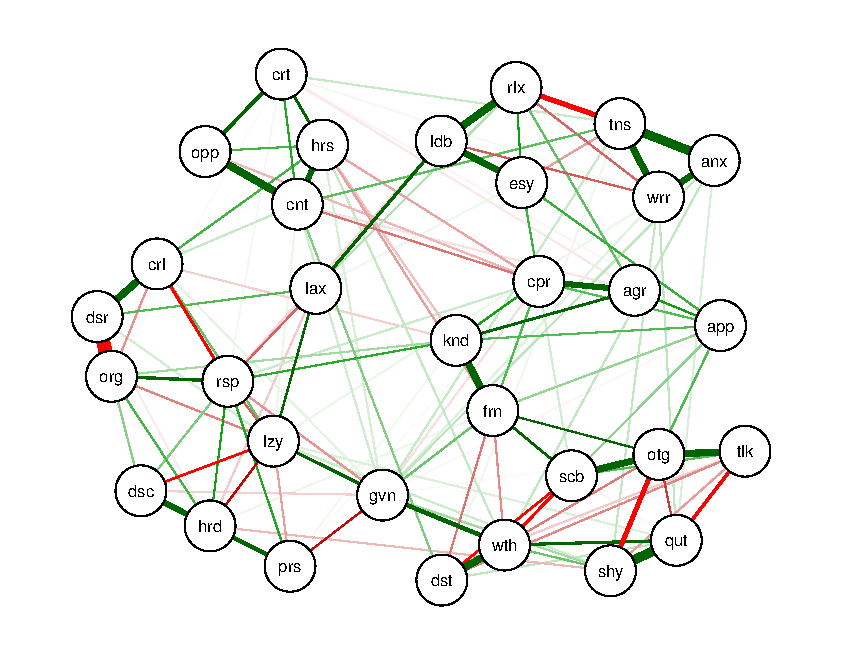
\includegraphics[scale=.9]{pics/personality_lasso}
%	\end{center}
%\end{frame}




\subsection{Log-linear models}

\begin{frame}[plain,noframenumbering]{}
\begin{center}
	{\huge \textcolor{DarkRed}{Log-linear models}}
\end{center}
\end{frame}


\begin{frame}{Hierarchical models}
Random vector $X=(X_1,\ldots,X_m)$ with state space $\cX=\cX_1\times \cdots\times \cX_m$,\quad  $|\cX_i|<+\infty$.\\[.3cm]
	\alert{Generators}: Denote by $\cC$ a set of subsets of $\{1,\ldots,m\}$.\\[.4cm]
	

	\begin{beamercolorbox}[wd=\paperwidth,sep=3pt]{important}
		\textbf{The model}: $p(x)\;=\;\prod_{C\in \cC} \phi_C(x_C)$, \;\;where $\phi_C>0$.
	\end{beamercolorbox}
	\bigskip
	
	\textcolor{SeaGreen}{Main effect model}: $\cC=\{\{1\},\ldots,\{m\}\}$.\\[.3cm]
	\textcolor{SeaGreen}{Pairwise interaction model}: $\cC=\{\mbox{all pairs}\}$.\\
	\qquad $\bullet$ more generally: edges of a graph with m nodes.\\[.3cm]
		\textcolor{SeaGreen}{Graphical models}: $\cC$ be the set of maximal cliques of $G$.\\[.3cm]
\end{frame}

%\begin{frame}{Graphical and non-graphical models}
%
%	Hammersley-Clifford theorem (Slide~\ref{HC}) gives equivalent description in terms of conditional independences of a discrete graphical model.\\[.3cm]
%		
%Two remarks:
%\begin{itemize}
%\item Both pairwise interaction models and graphical models are represented by graphs but the graphs encode different information. 
%	\item Every pairwise interaction model with underlying graph $G$ is contained in graphical model over $G$. (so the conditional independence information is retained)
%\end{itemize}
%\end{frame}

\begin{frame}[fragile]{Fitting log-linear models in \texttt{R}}
The function \texttt{loglin()} fits general log-linear models. We focus here on the ones represented by graphs, that is, graphical or pairwise. \\[.3cm]

The \texttt{gRim} package has a function \texttt{dmod()} to define and fit hierarchical log-linear models for a fixed set of generators. 	
\begin{lstlisting}
> data(lizard)
> mliz <- dmod(list(c("species","height"),c("species","diam")),data=lizard) 	
> mliz

Model: A dModel with 3 variables
 -2logL    :        1604.43 mdim :    5 aic :      1614.43 
 ideviance :          23.01 idf  :    2 bic :      1634.49 
 deviance  :           2.03 df   :    2 
\end{lstlisting}
{\small On \texttt{data(lizard)}: Behaviour characteristics of 409 lizards were recorded: species (\texttt{anoli}, \texttt{dist}), perch diameter (\texttt{<=4}, \texttt{>4}), and perch height (\texttt{>4.75},\texttt{<=4.75}).}
\end{frame}

%\begin{frame}{}
%	In case of non-hierarchical models use \texttt{glm()}.
%\end{frame}

\begin{frame}[fragile]{Testing conditional independence}
If the data is given in form of a contingency table it is convinient to use \texttt{gRim}'s \texttt{ciTest\_table}.
 
\begin{lstlisting}
> ciTest_table(lizard,set=c("height","diam","species"))
Testing height _|_ diam | species 
Statistic (DEV):    2.026 df: 2 p-value: 0.3632 method: CHISQ
Slice information:
  statistic p.value df species
1     0.178  0.6731  1   anoli
2     1.848  0.1741  1    dist


> ciTest_table(lizard,set=c("diam","species","height"))
Testing diam _|_ species | height 
Statistic (DEV):   14.024 df: 2 p-value: 0.0009 method: CHISQ
Slice information:
  statistic   p.value df height
1     2.903 0.0884377  1  >4.75
2    11.122 0.0008533  1 <=4.75
\end{lstlisting}
Notice the \texttt{df} calculation, which in general may be complicated.

\end{frame}
%> ciTest_table(lizard,set=c("height","species","diam"))
%Testing height _|_ species | diam 
%Statistic (DEV):   11.823 df: 2 p-value: 0.0027 method: CHISQ
%Slice information:
%  statistic  p.value df diam
%1     9.243 0.002364  1  <=4
%2     2.580 0.108239  1   >4


%\begin{frame}[fragile]{Decomposable graphs}
%	This is particularly useful if computations can be done locally for each $C_i$ and then glued back together.\\[.3cm]
%	This typically can be done as long as $G$ is \textbf{\alert{decomposable}}, that is, it has no induced cycles of length $\geq 4$. \\[.3cm]	
%	(write how to use R to check it)
%	
%	To generate a random decomposable graph write in R:
%	\begin{lstlisting}
%library(GLSE)	
%n <- 10
%edge <- 20
%A <-decGraph (n,edge) # Generate a decomposable graph.
%Graph <- graph_from_adjacency_matrix(A, mode = "undirected")
%plot(Graph)	
%	\end{lstlisting}
%\end{frame}


%\begin{frame}{Model selection}
%In general graphical lasso approach is hard to perform. \\
%\quad {\small $\bullet$ c.f. Ling-Loh, Wainwright, \textit{Structure estimation for discrete graphical models: Generalized covariance matrices and their inverses}}
%
%\bigskip
%Typical strategies:
%\begin{enumerate}
%	\item [(i)] using conditional independence tests,
%	\item [(ii)] heuristic search to optimize some information criterion,
%	\item [(iii)] Bayesian methods involving MCMC.
%\end{enumerate}
%\end{frame}

\begin{frame}[fragile]{Stepwise methods for discrete graphical models}
	For stepwise methods  typically the penalized likelihood criteria like BIC or AIC are used.\\[.3cm]
	Stepwise methods either start with the full graph or the empty graph.
		\begin{lstlisting}
> data(reinis); m.init <- dmod(~.^., data=reinis)
> m.reinis <- stepwise(m.init) # AIC criterion
> m.reinis.2 <- stepwise(m.init,k=log(sum(reinis))) # BIC criterion
> plot(m.reinis); plot(m.reinis.2)		
\end{lstlisting}
\begin{center}
	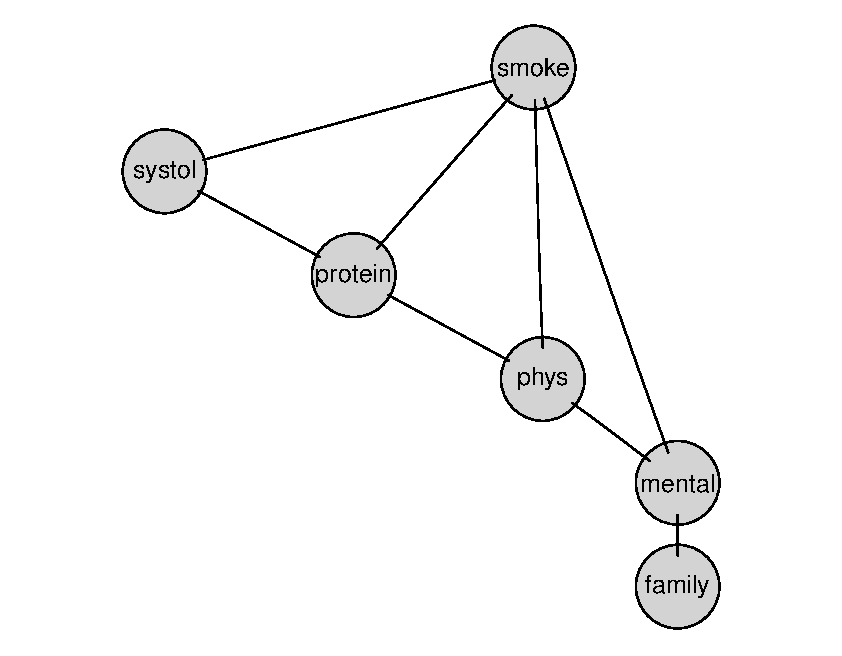
\includegraphics[scale=.3]{pics/reinis}\qquad\qquad 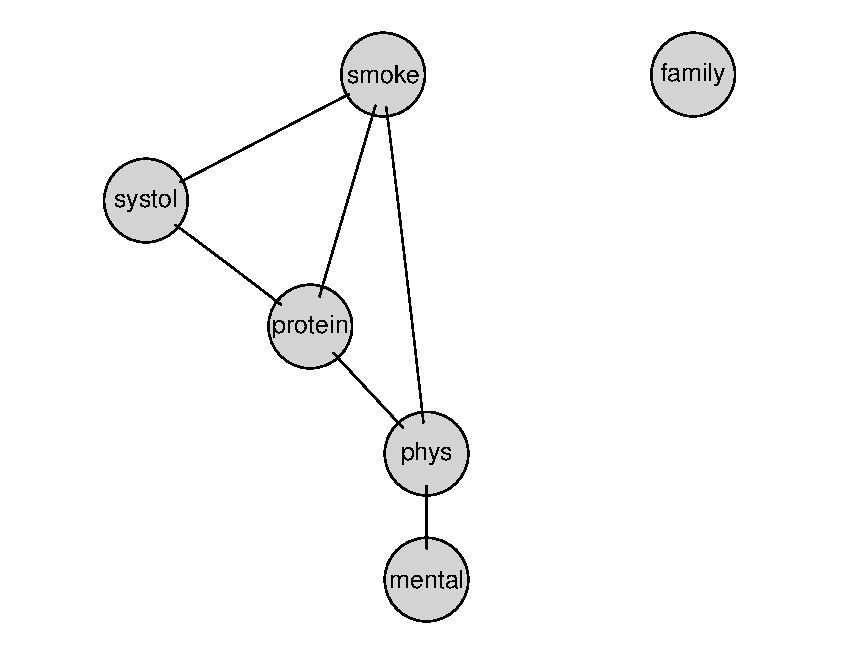
\includegraphics[scale=.3]{pics/reinis2}
\end{center}
\end{frame}

\begin{frame}{Modelling large data sets}
		\begin{beamercolorbox}[wd=\paperwidth,sep=3pt]{important}
With $>10$ variables stepwise methods are computationally prohibitive. 
	\end{beamercolorbox}
	\bigskip
	
Possible strategies:\\[.3cm]
\begin{enumerate}
	\item Use MCMC (\texttt{BDgraph} package)
	\item Focus on \alert{decomposable models} (\texttt{gRapHD} package).\\[.3cm]
	\item Rely on simpler models (e.g. pairwise interaction models). \\[.3cm]
	\item Restrict to very simple graphs (e.g. trees).
\end{enumerate}
\bigskip

\alert{This is an active research area.}
\end{frame}



\begin{frame}{Binary Ising model}
	Consider a log-linear model with only pairwise interactions.\\[.3cm]
	If $\cX=\{-1,1\}^m$ then $$f(x)\;=\;\tfrac{1}{Z(h,B)}\exp\left(\sum_i h_i x_i+\sum_{i<j}\beta_{ij}x_i x_j \right),$$
	where $h\in \R^m$ and $B=[\beta_{ij}]$ has zeros on the diagonal.\\[.3cm]
	Likelihood is hard to handle because $Z(h,B)$ is intractable if $m$ is large.\\
	\bigskip
	
	This will be our first encounter with pseudo-likelihood methods.
\end{frame}


\begin{frame}{Pseudo-likelihood approach}
\begin{block}{Logistic regression}
Denoting \textcolor{blue}{$\eta_k=h_k+\sum_{i\neq k}\beta_{ik}x_i$}, the full conditional distributions satisfy
	$$
	\log p(x_k|x_{-k})=\eta_k x_k-\log(e^{-\eta_k}+e^{\eta_k })
	$$ 
	and so, if $p= p(1|x_{-k})$, then \;\;\;\;\;
	$
	\log \frac{p}{1-p}\;=\;2\eta_k\;=\;2h_k+\sum_{i\neq k}2\beta_{ik}x_i.
	$
\end{block}
\begin{alertblock}{$\ell_1$-regularized logistic regression (Ravikumar et al, 2010)}
	Having observed $\x_1,\ldots,\x_n$, to learn the support of $B$, we can optimize for each $k$ the logistic regression given the data. Alternatively we can maximize
	$$
	\sum_{i=1}^n \sum_{k\in V} \log p(x_k^{(i)}|x_{-k}^{(i)})\;-\;\lambda \|B\|_1.
	$$
\end{alertblock}
\end{frame}

\begin{frame}[fragile,label=DepAnx]{Using \texttt{IsingFit}}
	\begin{lstlisting}
> install.packages("IsingFit"); library(IsingFit)
> ncsdata=read.table(file="./data/DepressionAnxiety.txt") 
> colnames(ncsdata)=c("depr", "inte", "weig", "mSle", "moto", "mFat", "repr", "conc", "suic", "anxi", "even", "ctrl", "edge", "gFat", "irri", "gCon", "musc", "gSle") #Define variable names.
# remove two variables that are perfectly correlated with each other in the sample
> X <- (ncsdata[,-(10:11)])
# run the high-dimensional Ising model selection problem
> Res <- IsingFit(X,gamma = 0.5, plot=FALSE)
# compare with the correlation network
> lay <-averageLayout(Res$weiadj,cor(X), layout = "spring", repulsion = 1)
> qgraph(cor(X),layout=lay,labels=colnames(X))
> qgraph(Res$weiadj, layout = lay)
# both graphs appear on the next slide
\end{lstlisting}
For a discussion of this dataset see:\\[.2cm]
{\footnotesize Borsboom and Cramer, Network analysis: an integrative approach to the\\[-.2cm] structure of psychopathology, Annual review of clinical psychology, 9 (2013). }
\end{frame}


\begin{frame}{Two psychological disorders}
\alert{About the study:}\\[.5cm]
National Comorbidity Survey Replication  (NCS-R data)\\[.4cm]
9282 observations of 18 binary variables such as:\\
\texttt{depr} (Depressed mood), \texttt{inte} (Loss of interest), etc\\[.4cm]
These are symptoms related to two disorders:\\ major depression and generalized anxiety disorder.\\[.4cm]
Bridge variables: sleep problems, fatigue, and concentration problems.

\end{frame}


\begin{frame}{Two psychological disorders, continued}
\alert{About the data:}\\[.5cm]
Sparse contingency table: $872/65536$ nonzero cells. \\[.4cm]
5667 out of 9282 respondents recorded no symptoms.\\[.4cm]
two variables perfectly correlated with each other and other seven variables.\\[.4cm]
\end{frame}



\begin{frame}[label=depr_lasso]{}
	\begin{center}
		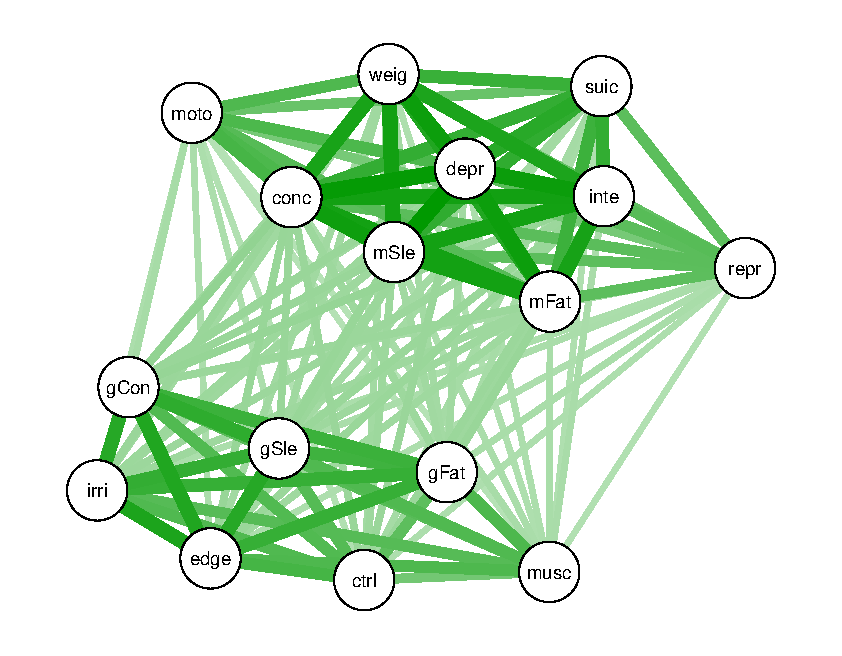
\includegraphics[scale=.5]{pics/depr_corr}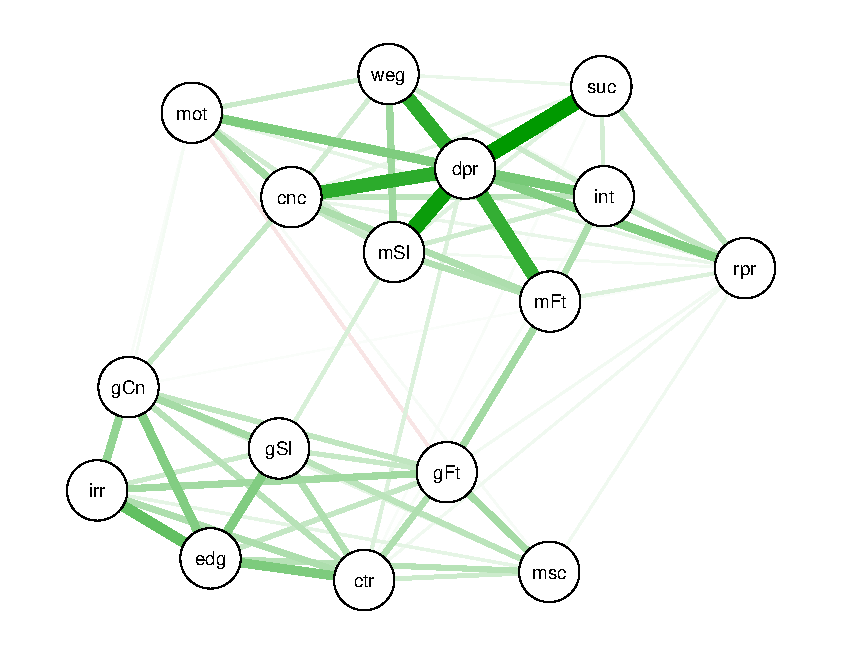
\includegraphics[scale=.5]{pics/depr_lasso}
	\end{center}
\end{frame}


\section{Beyond the standard set-up}

\begin{frame}[plain,noframenumbering]{}
\begin{center}
	{\Huge \textcolor{DarkRed}{Gaussian copula graphical models}}
\end{center}
\end{frame}


\begin{frame}[label=npn]{Nonparanormal distributions}
	$(X_1,\ldots,X_m)$ has \textcolor{blue}{nonparanormal} distribution if $(f_1(X_1),\ldots,f_m(X_m))$ is Gaussian $N(\mu,\Sigma)$ for some monotone functions $f_1,\ldots,f_m$.
	\begin{itemize}
		\item This is the same as the Gaussian copula model; thus assume $\mu=0$, $\Sigma_{ii}=1$.
	\end{itemize}	
The functions $f_i$ are treated as nuisance parameters. The correlation matrix is estimated directly using \textcolor{blue}{rank correlation statistics}:\\[.2cm]
	\begin{alertblock}{We can estimate the correlation matrix of $f(X)$ without knowing f!!}
		If $\tau_{ij}={\rm cor}(\sgn(X_i-X_i'),\sgn(X_j-X_j'))$ is the \textcolor{blue}{Kendall's tau coefficient} then
	$$
	\Sigma_{ij}:={\rm cor}(f(X_i),f(X_j))\;=\;\sin\left(\tfrac{\pi}{2}\tau_{ij}\right).
	$$
	\vspace{-.8cm}
	\begin{itemize}
		\item $\tau_{ij}$'s are invariant under monotone transformations on $X_i$'s.
	\end{itemize}
	\end{alertblock}
Note that graphical models for $X$ and $f(X)$ are identical.
\end{frame}


\begin{frame}[label=npn2]{Estimating nonparanormal graphical models}
		Compute \alert{Kendall's tau} coefficients from the data (c.f. Slide~\ref{tau}).\\[4mm] 	
		Define $\hat S^\tau=\sin(\tfrac{\pi}{2}\hat\tau_{ij})$.\\[.3cm]
	Concentration analysis based on U-statistics shows that
	$$
	\max_{ij}|\hat S^\tau_{ij}-\Sigma^0_{ij}|=\mathcal O\left(\sqrt{\tfrac{\log(mn)}{n}}\right).
	$$
	\begin{beamercolorbox}[wd=\paperwidth,sep=5pt]{important}
		Based on $\hat S^\tau$ we can now employ any standard Gaussian procedure to learn the graph, e.g., graphical lasso.
	\end{beamercolorbox}

\end{frame}

\begin{frame}[fragile]{Application using \texttt{huge} package}

{\small Stock market data: closing prices from all stocks in the S\&P 500 for all the days that the market was open between Jan 1, 2003 and Jan 1, 2008. }
	\begin{lstlisting}
> library(huge); data(stockdata) # Load the data 
> x = log(stockdata$data[2:1258,]/stockdata$data[1:1257,]) # Preprocessing 
> colnames(x) <- stockdata$info[,1]
> x.npn = huge.npn(x, npn.func="skeptic") # Nonparanormal + Kendal's tau
> out.npn = huge(x.npn,method = "glasso")
> plot(out.npn)
# plot the graph corresponding to lambda=0.397
> Khat <- (out.npn$icov[[15]]+t(out.npn$icov[[15]]))/2; colnames(Khat) <- rownames(Khat) <- colnames(x)
> dev.off(); qgraph::qgraph(-cov2cor(Khat),layout="spring")
\end{lstlisting}
	This is a rather large example to be handled by \texttt{qgraph} directly.
	\begin{lstlisting}
> qgraph(x.npn,graph="glasso",sampleSize=nrow(x),layout="spring")
\end{lstlisting}

	{\scriptsize Zhao, T., Liu, H., Roeder, K., Lafferty, J., \& Wasserman, L. (2012). The huge package for high-dimensional undirected graph estimation in R. Journal of Machine Learning Research.}
\end{frame}

\begin{frame}{}
The non-paranormal approach gives:
\begin{center}
	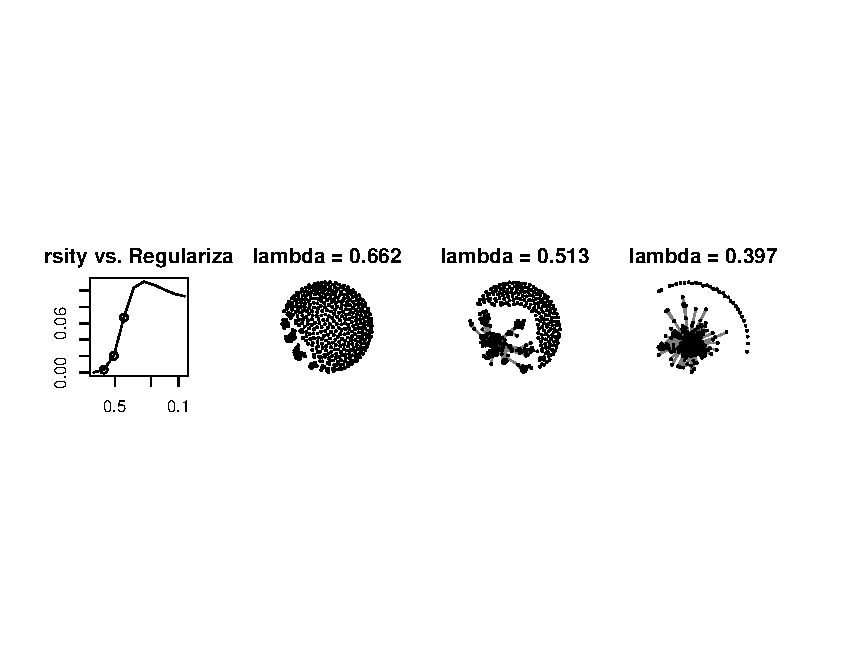
\includegraphics{pics/huge_stocks1}	
\end{center}
For comparison a direct Gaussian approach gives:
\begin{center}
	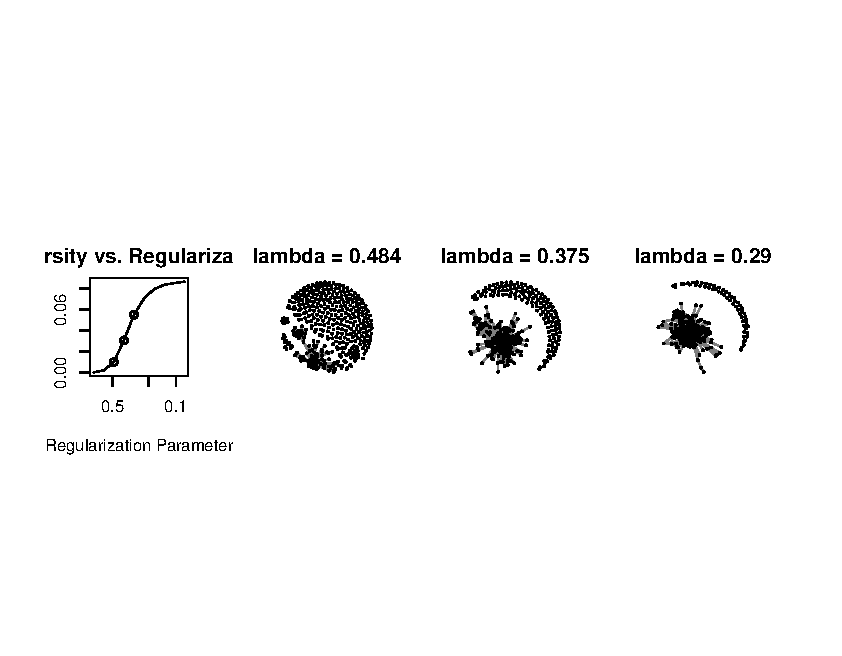
\includegraphics{pics/huge_stocks1_gauss}	
\end{center}
\end{frame}

\begin{frame}{}
\begin{center}
	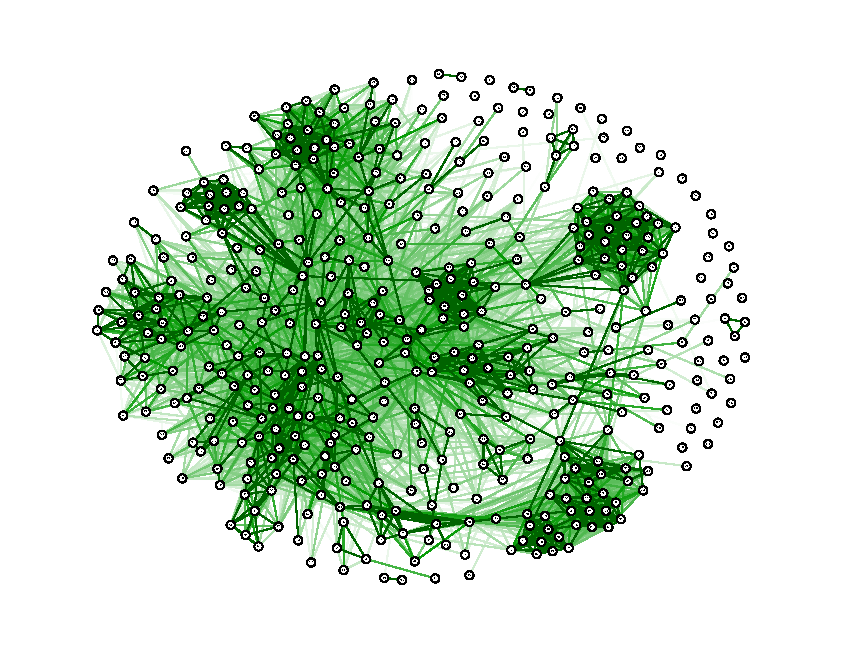
\includegraphics[scale=.8]{pics/huge_stocks2}	
\end{center}
\end{frame}



\end{document}

